\documentclass[output=paper]{langscibook}
\ChapterDOI{10.5281/zenodo.5578840}

\author{Madeleine Oakley\affiliation{Georgetown University}}


\title{Acoustic correlates to contrastive tone heights in two African languages}  
\abstract{\sloppy Languages with contrastive tone may phonetically realize tonal distinctions through changes in F0, relative F0, and vowel duration, amongst other cues \citep{abramson1979, zhang2001, levi2005, brunelle2016, alan2010}. It has been argued that there is a universal correlation between vowel duration and F0, where H tones correspond to short vowels, and L tones correspond to long vowels  \citep{abramson1979, dreher1968instrumental, gandour1977interaction}. This pilot study expands the study of acoustic correlates of tonal contrasts by examining the interaction of pitch and duration in two understudied African languages: Nobiin and Guébie. The pilot study results do not show evidence for a negative correlation between pitch and vowel duration, suggesting this presumed universal correlation may be language (or even speaker) specific. Furthermore, the acoustic correlates to tone are independent of the phonological inventories of Nobiin and Guébie, which has implications for the phonetics/phonology interface.} 


\begin{document}
\SetupAffiliations{mark style=none}
\maketitle

\section{Introduction}\label{sec:oakley:1}

Lexical tone contrast may have multiple acoustic correlates. Lexical tone may be realized by relative F0, changes in F0, or vowel length, amongst other phonetic cues \citep{abramson1979, zhang2001, levi2005, brunelle2016, alan2010}.  It has been suggested that universal phonetic properties influence the relationship between F0 and vowel duration. Many studies have found a negative correlation between F0 and vowel duration: high tones correlate to shorter vowel durations, while low tones are correlated with longer vowels in Thai, Mandarin, and Medʉmba \citep{gandour1977interaction, dreher1968instrumental, franich2016internal}. Recently, however, the universality of this negative correlation has been questioned. Studies looking at languages with level tone have found a positive correlation between F0 and vowel duration, suggesting that the assumed universal correlation between F0 and vowel duration may be a language specific property rather than a universal phonetic constraint \citep{alan2010, Mamadou2018, Kpodo2018}. Additionally, it has been argued that the phonological system of a language will impact what phonetic units are used to cue prominence \citep{remijsen2014study}. A language may not use vowel length to cue stress if vowel length is contrastive in the language. The present work is a pilot study that examines the relationship between vowel length and tone in two underdocumented African languages, Nobiin (Nilotic) and Guébie (Kru).

\subsection{Acoustic correlates of tone}
\begin{sloppypar}
Multiple acoustic features may correlate to tone or stress, which serves to optimize the prominence of the unit. Stress is argued to be realized primarily through vowel lengthening, while tone is realized primarily through F0 \citep{remijsen2014study, lunden2017vowel}. However, in languages such as Washo, Welsh, and Zapotec that have contrastive vowel length in addition to stress, other acoustic cues besides vowel lengthening will be primarily used as acoustic correlates to prominence \citep{remijsen2014study}. If a language has contrastive vowel duration, vowel length may not be optimal to cue stress \citep{berinstein1979cross, remijsen2014study}. This implies that the acoustic correlates to prominence may be predictable based on the phonological system of a language, as optimal phonetic correlates to prominence may be in a one-to-one relationship with phonological information. The present study expands on this work to look at the acoustics of tone, rather than stress.
\end{sloppypar}

\subsection{Relationship between acoustic correlates of tone}
Studies investigating the relationship between the acoustic correlates of tone and prominence have suggested that there may be a universal relationship between acoustic correlates and tone. H tones tend to be short, while L tones tend to be long. Evidence for a negative correlation between F0 and vowel duration comes from studies examining perception or production data from Thai, Mandarin, and Medʉmba, among others \citep{gandour1977interaction, dreher1968instrumental, franich2016internal}. Thai has contrastive vowel length and contrastive tone. However, vowel length has been lost in certain Thai dialects. Gandour argues that the loss of the phonological distinction of contrastive long vowels is conditioned by tone \citep{gandour1977interaction}. \cite{gandour1977interaction} argues that the negative correlation between vowel duration and average F0 of tones in Thai may be physiologically motivated, which can additionally condition sound change. 

Perception studies have largely supported the claim that F0 and vowel duration are inversely related. In one such study, speakers of Medʉmba participated in a word identification task, and results show that vowels with short durations and low F0 were more likely to be identified as H tones than vowels with longer durations \citep{franich2016internal}. These results expand the claim that there may be a universal negative correlation between vowel duration and F0 by looking at perception data from a level-tone language. However, Medʉmba does not have contrastive vowel length, meaning duration is exclusively used as a cue to tonal contrasts. The present study will further address how vowel length and pitch interact, specifically by looking at a language that has contrastive vowel length and two level tones (Nobiin), and a language with no contrastive vowel length and four contrastive tones (Guébie).

The studies addressed above have found production and perception data to support the claim that vowel duration and F0 can be used as acoustic cues to tonal contrasts in both contour tone and level tone languages. However, recent studies looking at tone production in various level tone languages have shown evidence for a \textit{positive} correlation between pitch and duration. In one such study, acoustic data from speakers of Ewe and Ga (both Kwa languages that have level and contour tones, and no contrastive vowel length) shows that F0 and vowel duration are positively correlated \citep{Kpodo2018}. Similarly, acoustic data from speakers of Yoruba (a language with three level tones and no contrastive vowel length) finds that vowels on H tones have a longer duration than M or L tone vowels \citep{Mamadou2018}. This calls into question whether or not the negative correlation between pitch and duration found in many languages is physiological (and thus universal).

\subsection{Phonological inventory of Nobiin and Guébie}
The present analysis is a pilot study, which expands on work addressing the relationship between pitch and vowel duration to two underdocumented African languages; Nobiin and Guébie. Nobiin is a Nilo-Saharan language spoken in southern Egypt and northern Sudan. Because of geopolitical reasons, many Nobiin speakers have been displaced. Nobiin has two contrastive level tones: H and $\emptyset$. On the surface, $\emptyset$ is realized as L. Minimal pairs show level tone is lexically contrastive in Nobiin: 


\ea \label{ex:oakley:NobiinContrastiveTone}
\begin{xlist}

\ex \label{ex:oakley:NobiinElder}
\gll /daww\'i/ \\
elder \\
\glt `elder' 

\ex \label{ex:oakley:NobiinPath}
\gll /dawwi/ \\
path \\
\glt `path' 

\end{xlist}

\z 



Nobiin has five short vowels and five long vowels: /i, i:, e, e:, a, a:, u, u:, o, o:/. All of the vowels can bear a H or L tone.

Guébie is a Kru language spoken by around 7,000 speakers in southwest C\^ote d'Ivoire. Guébie has four contrastive level tones, labeled here as tones 1--4, 1 being the low tone and 4 being the high tone \citep{sande2017}. Contour tones are also contrastive in Guébie, with tone melodies 41, 31, 42, 32, 13, 23, and 24 attested. However, contour tones are not examined in the present study, as the primary goal is to compare the acoustic correlates to level tone in Nobiin and Guébie. There are 10 contrastive vowels in Guébie, /i, e, ɛ, u, ʊ, o, ɔ, ə, a/, and vowel length is not contrastive \citep{sande2017}.


This study seeks to answer the following research questions:
\begin{enumerate}
\item How does vowel length interact with tone? 

In languages that have tone and phonemic vowel length (Nobiin), do H tones have shorter vowel durations than L tones? Do short vowels have higher F0 than long vowels?

\item What are the acoustic correlates to tone in Nobiin and Guébie?

Do languages with contrastive vowel length (Nobiin) also use vowel length to distinguish tonal contrasts? Does this differ from languages without contrastive vowel length (Guébie)?

\item Do Nobiin and Guébie show evidence for a negative or positive correlation between F0 and vowel duration?
\end{enumerate}

Acoustic production data from two speakers of Nobiin and two speakers of Guébie are examined in this pilot study. Although a small number of speakers are included, both Nobiin and Guébie have very little acoustic-phonetic data available. Nobiin is classified as a threatened language \citep{570887}, and many speakers have been displaced. Due to the political nature of this displacement, little documentation work has been undertaken. This study provides phonetic data of tone in Nobiin, which has previously not been available. Additionally, Guébie is an endangered language, with little recorded phonetic data. Nearly all speakers of Guébie are bilingual, and learn French from an early age. Because of cultural considerations of working in the community, few recordings are available that are suitable for phonetic analysis, thus highlighting the importance of this current description, despite the small number of speakers. 

\section{Methods}
\subsection{Nobiin speakers' production task} 

Two Nobiin speakers were recorded in Washington, D.C. in a quiet classroom. Both speakers are male and between the ages of 40 and 60. For the production task, a word list was designed to elicit H and L tones on vowels in object position. The word list controlled for vowel quality to the extent possible. Items on the word list had all ten Nobiin vowels with H and L tone. While an effort was made to include a token of H and L vowels for every Nobiin vowel, a few gaps remain. The present study does not include L tone tokens of /o/. 


Participants were given the lexical item in English and asked to translate it into Nobiin. Each word was produced in the carrier phrase shown in \REF{ex:oakley:NobiinCarrierPhrase}.


\ea \label{ex:oakley:NobiinCarrierPhrase}
\gll  aj “X” igitis\\
\textsc{1sg} “X” say.\textsc{1sg}\\
\glt  `I say “X”{}'
\z

The target word “X” in each carrier phrase was analyzed. Participants repeated this phrase three times, and one token of each lexical item was selected for analysis. A total of 82 vowels are included in the present study. Recordings were made using a Zoom H4n recorder and a lavalier microphone. 

Acoustic measurements were made in Praat \citep{Boersma2017}. F0 was measured at three evenly spaced measurement points throughout the duration of the vowel: the first measurement point (T1) was taken at 1/3 of the vowel duration, the second (T2) at 1/2 of the vowel duration, and the final measurement point (T3) was taken at 2/3 of the duration of the vowel. The first third and last third of the vowel was not measured to avoid the effects of consonant voicing on F0 to the extent possible. 

Pitch slope was measured over the middle 1/3 of the vowel. Slope was calculated for each vowel by subtracting F0 (in Hz) at time T1 from the F0 value (in Hz) at time T3. This value was then divided by the duration of the vowel (in ms). This measurement provides information about how pitch changes throughout the duration of the vowel.


Vowel duration of each target vowel was measured in milliseconds. In order to control for the speech rate of each utterance, vowel duration was measured as a ratio with the pronoun in the subject position. Thus, the duration of the pronoun [aj] was measured in milliseconds for each phrase, and the duration of the target vowel was divided by the duration of the pronoun. The results report duration as a ratio value. 

First, pitch measurements taken across the vowel duration were compared using $t$-tests in order to describe the phonetics of tone in Nobiin. To address the first research question, a factorial ANOVA comparing vowel duration for phonemically short and long vowels, and H and L tones was conducted to both describe the phonetic correlates to vowel length, and investigate the interaction between tone and vowel duration. A separate factorial ANOVA comparing F0 at the vocalic midpoint for H and L tones, and long and short vowels, was included to further address research question 1. Next, to address research question 2 regarding the acoustic correlates to tone, a logistic mixed-effects model was run, with tone identity as the dependent variable, and pitch and vowel duration measures as fixed-effects. This analysis shows which acoustic factors distinguish contrastive tone in Nobiin. Finally, to address research question 3 regarding the relationship between acoustic correlates to tone, a correlation analysis was run for each Nobiin speaker, to see how pitch and (phonetic) vowel duration correlate. This analysis serves to examine whether the current data supports the presumed universal negative correlation between pitch and vowel duration. Results are presented in \sectref{sec:oakley:Results}.

\subsection{Guébie speakers' production task}
\begin{sloppypar}
Two Guébie speakers were recorded in Gnagbodougnoa, C\^ote d'Ivoire. Both speakers are male and between the ages of 30 and 45. Due to constraints on resources in the field work setting, recording sessions took place in quiet locations outside of homes. For the production task, target words were chosen to elicit every combination of vowel and tone pairs. The word list controlled for the voicing on the preceding and following consonants to the extent possible. 
\end{sloppypar}

Speakers were given a phrase in French and asked to translate the phrase into Guébie. All of these phrases had the third person singular pronoun [ɔ] in the subject position. Carrier phrases were not used in elicitations because of cultural considerations of collecting data in Gnagbodougnoa. All phrases were repeated three times, and one lexical item in phrase medial position was selected for analysis. Because recordings were not made in a quiet lab-like setting, tokens were only chosen if they had minimal background noise. A total of 453 tokens are thus included in the present analysis. Again, recordings were made using a Zoom H4n recorder and a lavalier microphone. 

The same acoustic measurements described above were also analyzed for Guébie speakers in PRAAT. For vowel duration, the duration of the pronoun [ɔ] was measured in milliseconds for each phrase, and the duration of the target vowel was divided by the duration of the pronoun. All other acoustic measurements are consistent for Nobiin and Guébie speakers.

Pitch measurements taken at three points across the vowel duration were compared using ANOVAs. Next, to address research question 2, a logistic mixed-effects models was run, with tone identity as the dependent variable, and pitch and vowel duration measures as fixed-effects. The purpose of this analysis is to determine the acoustic correlates to pitch in Guébie, which has yet to be documented. Finally, a correlation analysis was run for each speaker comparing pitch and vowel duration, in order to determine whether these two phonetic measures are negatively correlated in Guébie, as predicted by previous literature.

\section{Results}\label{sec:oakley:Results}\label{sec:oakley:3}
\subsection{Nobiin acoustic results}
First, F0 at three time points was measured for all vowels and compared across H and L tones. F0 at each of the three time points was averaged (see \cite{svantesson2006} for similar methods), and compared for H and L tones. \figref{fig:oakley:TanutPitchTones} and \figref{fig:oakley:TonePitchNuban} show F0 throughout the duration of the vowel for Speaker 1 and Speaker 2 respectively. 

\begin{figure}
 \begin{floatrow}
  \captionsetup{margin=.05\linewidth}
   \ffigbox
     {\caption{F0 measurements during the middle 1/3 of vowel duration for H and L tones produced by Nobiin Speaker 1}\label{fig:oakley:TanutPitchTones}}
     {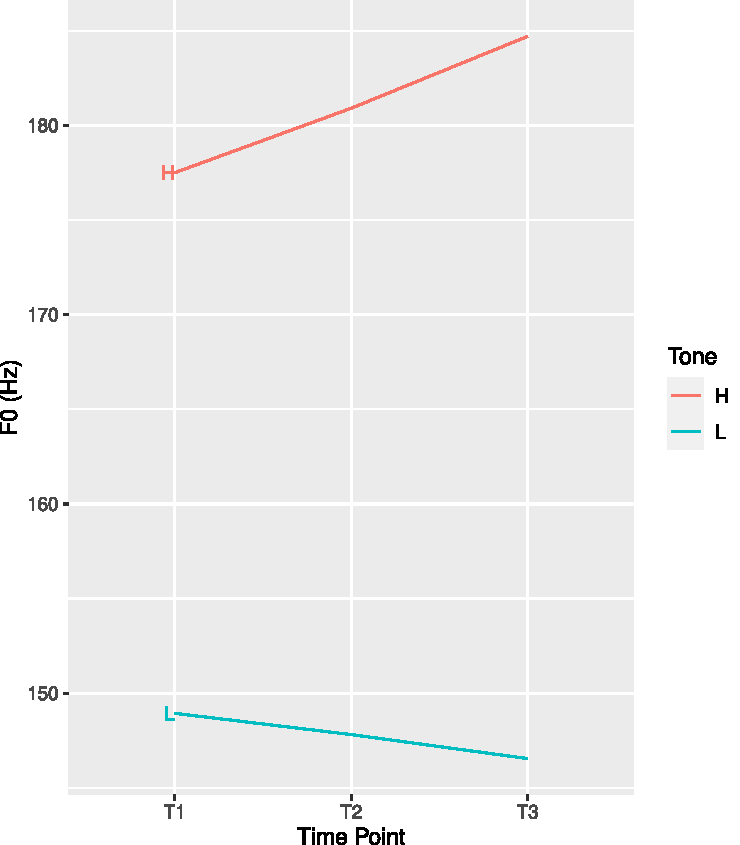
\includegraphics[width=.5\textwidth]{figures/TanutF0Movement.pdf}}%
   \ffigbox
     {\caption{F0 measurements during the middle 1/3 of vowel duration for H and L tones produced by Nobiin Speaker 2\label{fig:oakley:TonePitchNuban}}}
     {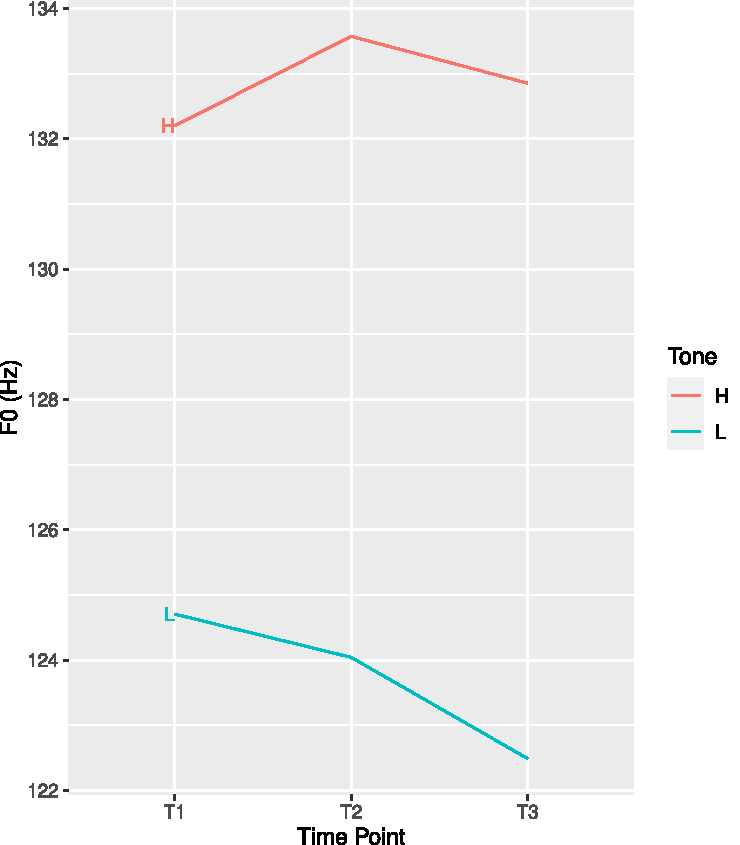
\includegraphics[width=.5\textwidth]{figures/NubanF0Movement.pdf}}
 \end{floatrow}
\end{figure}

\figref{fig:oakley:TanutPitchTones} and \figref{fig:oakley:TonePitchNuban} show, as expected, that H tones have a higher average F0 at each time point compared to L tones. $t$-tests at each time point for each speaker are shown in \tabref{tab:oakley:F0MovementTTest}, and confirm that H tones have significantly higher F0 values at T1, T2, and T3. Additionally, F0 tends to increase over the duration of the vowel for H tones (for both Speakers 1 and 2), and F0 decreases over the duration of the vowel for L tones.


\begin{table}
\caption{$t$-test results comparing average F0 of H and L tones at three different time points throughout the duration of the vowel\label{tab:oakley:F0MovementTTest}}
\begin{tabular}{l *{3}{S[table-align-text-after=false,table-align-exponent=false,table-format=1.4e1{***}]}}
\lsptoprule
          & {T1} & {T2} & {T3}\\ 
\midrule
Speaker 1 & 2.44e-6{***}& 1.16e-6 {***} & 5.52e-7 {***}\\ 
Speaker 2 & 0.018{*}& 0.0043 {**} & 0.0048 {**}\\ 
\lspbottomrule
\end{tabular}
\end{table}

Next, vowel duration was compared for phonemically short and long vowels, and for H and L tones, in order to examine how phonetic vowel duration varies according to phonological tone and vowel length. A factorial ANOVA with vowel duration as the dependent variable, and tone and phonemic vowel length as independent variables was used to compare vowel length for these contrasts. Two separate ANOVAs were conducted for Speaker 1 and Speaker 2, and results can be seen in \figref{fig:oakley:TanutVowelDur} and \figref{fig:oakley:NubanVowelDur}.

\begin{figure}
 \begin{floatrow}
  \captionsetup{margin=.05\linewidth}
   \ffigbox
     {\caption{Vowel duration for phonemically short and long vowels, and H and L tones, produced by Nobiin Speaker 1\label{fig:oakley:TanutVowelDur}}}
     {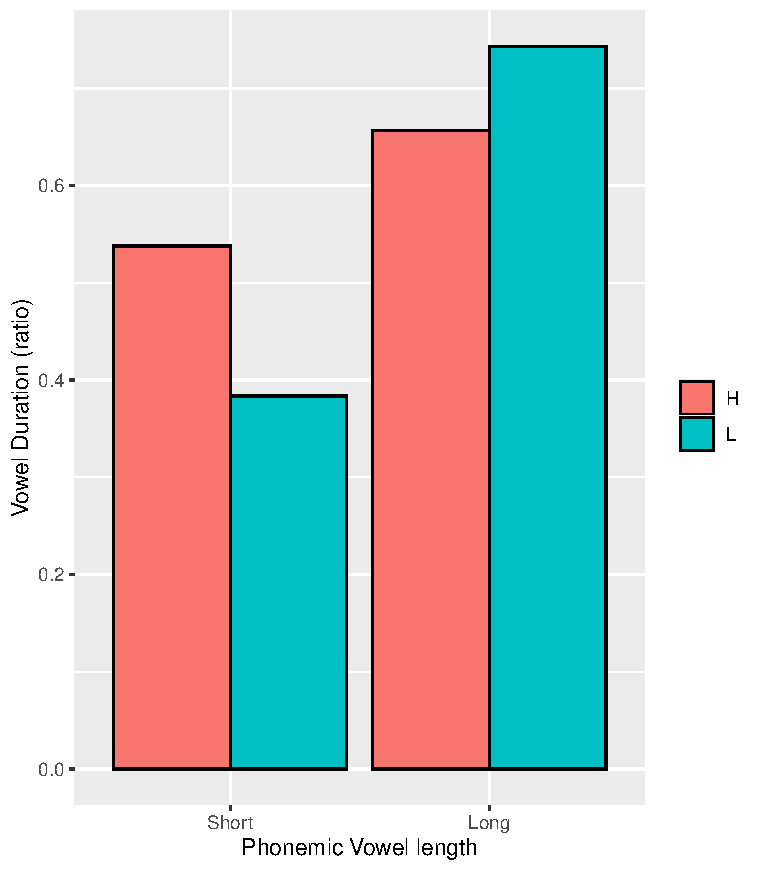
\includegraphics[width=.5\textwidth]{figures/TanutVowelDurBar.pdf}}%
   \ffigbox
     {\caption{Vowel duration for phonemically short and long vowels, and H and L tones, produced by Nobiin Speaker 2\label{fig:oakley:NubanVowelDur}}}
     {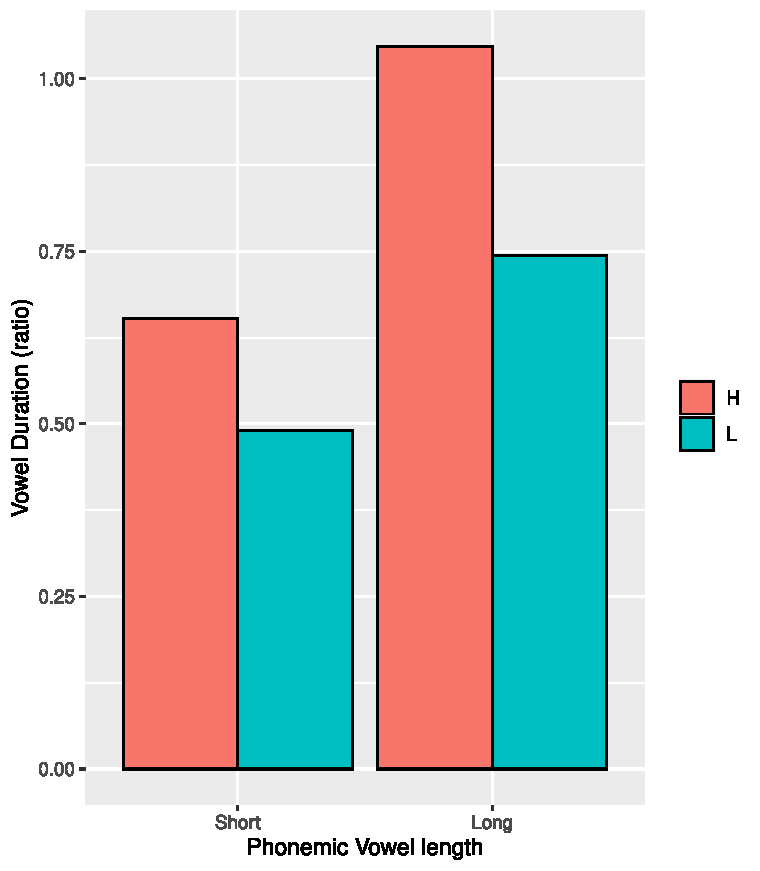
\includegraphics[width=.5\textwidth]{figures/NubanVowelDurBar.pdf}}
 \end{floatrow}
\end{figure}

For Speaker 1, there is a main effect of phonemic vowel length on vowel duration ($F=20.159; p=\num{5.28e-5}$***), and a marginal effect of the interaction between tone and vowel length on vowel duration ($F=3.83; p=0.056$). There is no effect of tone on vowel duration ($F=0.30; p=0.584$). Long vowels produced by Speaker 1 are longer in duration than short vowels (as expected). H tones also tend to be longer in phonemically short vowels than L tones, but H tones are shorter than L tones in phonemically long vowels. 

For vowel duration for Speaker 2, there is a main effect of phonemic vowel length on duration ($F=6.577; p=0.015$*), showing phonemically long vowels have a longer duration than short vowels. There is also a main effect of tone on vowel duration ($F=5.179; p=0.029$*). H tones tend to have a longer duration than L tones, for both phonemically long and short vowels. There is no effect on the interaction between tone and vowel length on vowel duration ($F=0.274; p=0.605$).

Having confirmed that contrastive vowel length does, in fact, correspond to longer vowel duration in Nobiin, the interaction of phonemic vowel length and tone on F0 was measured. Two factorial ANOVAs, one for each speaker, was run with F0 at the vowel midpoint as the dependent variable, and tone and vowel length as the independent variables. Results for Nobiin Speaker 1 show a significant main-effect of tone on F0 ($F=35.26; p=\num{4.49e-7}$***), and no significant effect of vowel length ($F=0.057; p=0.812$) or the interaction of tone and vowel length ($F=0.064; p=0.802$). The results for Nobiin Speaker 1 are shown in \figref{fig:oakley:TanutLengthToneInteraction}. Nobiin Speaker 2 shows the same pattern. There is a main-effect of tone on F0 at the vowel midpoint ($F=8.061; p=0.0079$**), and no effect of vowel length ($F=0.013; p=0.91$) or the interaction between vowel length and tone ($F=0.167; p=0.685$). These results are shown in \figref{fig:oakley:NubanLengthToneInteraction}.


\begin{figure}
 \begin{floatrow}
  \captionsetup{margin=.05\linewidth}
   \ffigbox
     {\caption{F0 of H and L tones at the vocalic midpoint, for short and long vowels, produced by Nobiin Speaker 1\label{fig:oakley:TanutLengthToneInteraction}}}
     {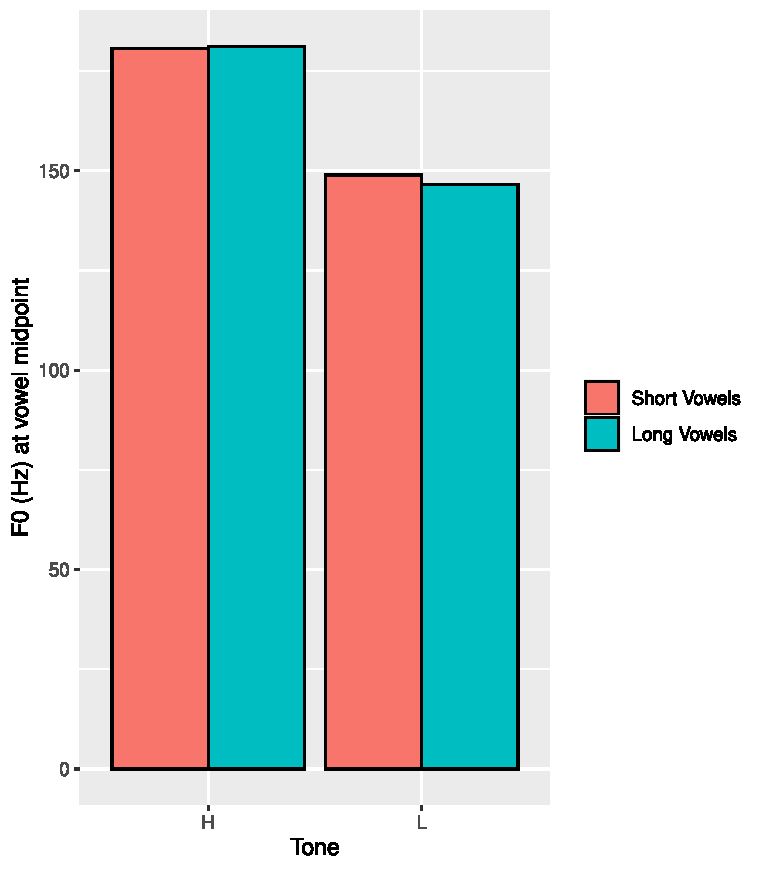
\includegraphics[width=.5\textwidth]{figures/TanutPitchlength.pdf}}%
   \ffigbox
     {\caption{F0 of H and L tones at the vocalic midpoint, for short and long vowels, produced by Nobiin Speaker 2\label{fig:oakley:NubanLengthToneInteraction}}}
     {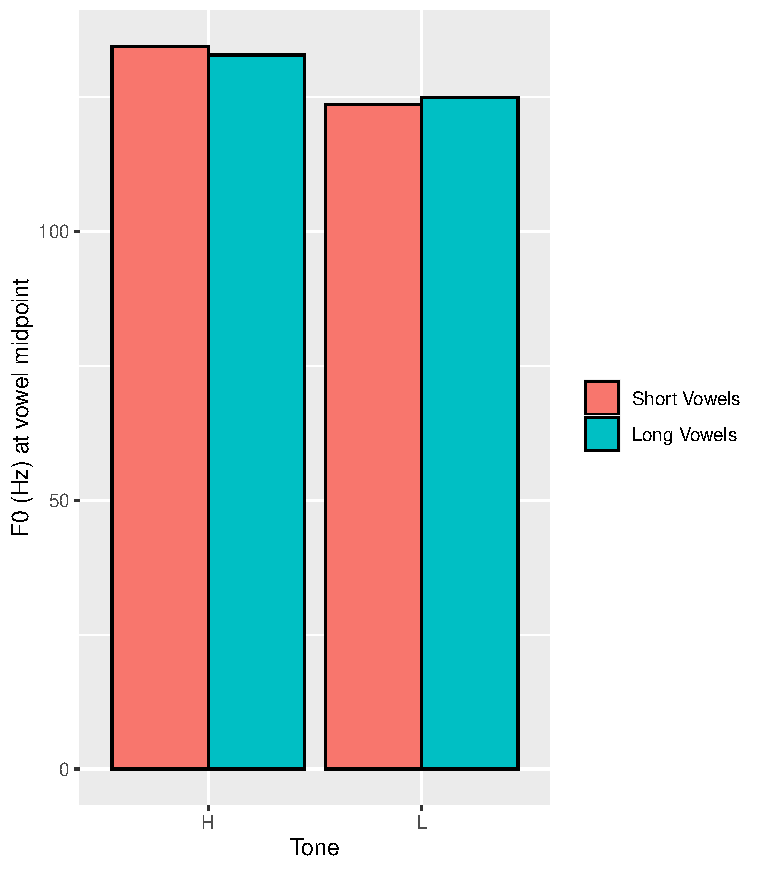
\includegraphics[width=.5\textwidth]{figures/NubanToneLengthFact.pdf}}
 \end{floatrow}
\end{figure}

These results show that phonemic vowel length does not effect pitch measurements. Long vowels and short vowels have very similar pitch measurements for H and L tones. Next, a logistic regression model was run in order to see the effects of \textit{phonetic} factors on predicting tone identity.

Two logistic mixed-effect regression models were run with tone type as the dependent variable; one model was run for short vowels, and one model was run for long vowels. Separate models were run for phonemically short and long vowels to only examine which phonetic factors are significant in predicting tone identity, while controlling for phonemic vowel length. For both models, F0 at the vowel midpoint, vowel duration, and F0 slope were included as fixed effects. F0 at the vowel midpoint was included as a measure of pitch to avoid the effects on pitch of surrounding consonants, to the extent possible. Random effects included speaker, vowel quality, and preceding consonant voicing. \tabref{tab:oakley:shortvowelmodel} shows the predictors that were significant from the models in predicting tone identity.

\begin{table}
\caption{Acoustic factors that influence tone identity; output of logistic-regression models for Nobiin speakers' productions of phonemically \textit{short} and \textit{long} vowels\label{tab:oakley:shortvowelmodel}\label{tab:oakley:longvowelmodel}}
\begin{tabular}{l S[table-format=1.3] S[table-format=1.3]}
 \lsptoprule
               & \multicolumn{2}{c}{$p$} \\\cmidrule(lr){2-3}
 Fixed-effect  & {short vowels} & {long vowels}\\\midrule
F0 at vowel midpoint & 0.017* & 0.075  \\ 
Pitch slope & 0.844           & 0.352  \\ 
Vowel Duration & 0.132        & 0.483  \\ 
\lspbottomrule
\end{tabular}
\end{table}

% % % \begin{table}
% % % \caption{Acoustic factors that influence tone identity; output of logistic-regression model for Nobiin speakers' productions of phonemically \textbf{long} vowels\label{tab:oakley:longvowelmodel}}
% % % \begin{tabular}{l S[table-format=1.3]}
% % %  \lsptoprule
% % % Fixed-effect  & {$p$} \\ 
% % % \midrule
% % % F0 at vowel midpoint & 0.075  \\ 
% % % Pitch slope          & 0.352  \\ 
% % % Vowel Duration       & 0.483  \\ 
% % % \lspbottomrule
% % % \end{tabular}
% % % \end{table}

The outputs of the regression models show slightly different patterns for short and long vowels in Nobiin. \tabref{tab:oakley:shortvowelmodel} shows for phonemically short vowels, F0 at the vowel midpoint is a significant predictor of whether a tone is H or L. Vowel duration and pitch slope are not significant in the model as predictors of tone. For phonemically long vowels, \tabref{tab:oakley:longvowelmodel} shows that F0 at the vowel midpoint is only significant at the 0.1 level in predicting whether a tone is H or L. Similar to short vowels, pitch slope and vowel duration are not significant factors in predicting tone identity for phonemically long vowels.

Finally, Pearson's correlation was used to examine the relationship between F0 at the midpoint of the vowel and vowel duration. The midpoint was chosen for the pitch measurement in order to avoid influence from the preceding and following segments on F0. Again, phonemically short and long vowels were measured separately because vowel length is contrastive in Nobiin, and is thus controlled for in order to only examine the interaction between \textit{phonetic} vowel duration and pitch. The two speakers were also measured separately, due to individual differences seen in the data. \figref{fig:oakley:TenutShortVowelsPitchvsDuration} and \figref{fig:oakley:TenutLongVowelsPitchvsDuration} show (respectively) the correlation between F0 and vowel duration for Speaker 1's phonemically short and long vowels, and \figref{fig:oakley:NubanShortVowelsPitchvsDuration}, and \figref{fig:oakley:NubanLongPitchvsDuration} show (respectively) the correlation between vowel duration and mean F0 for Speaker 2's phonemically short and long vowels.   

\begin{figure}
   \begin{floatrow}
     \captionsetup{margin=.05\linewidth}
     \ffigbox
     {\caption{Nobiin Speaker 1: correlation between mean F0 and vowel duration for phonemically short vowel productions\label{fig:oakley:TenutShortVowelsPitchvsDuration}}}
     {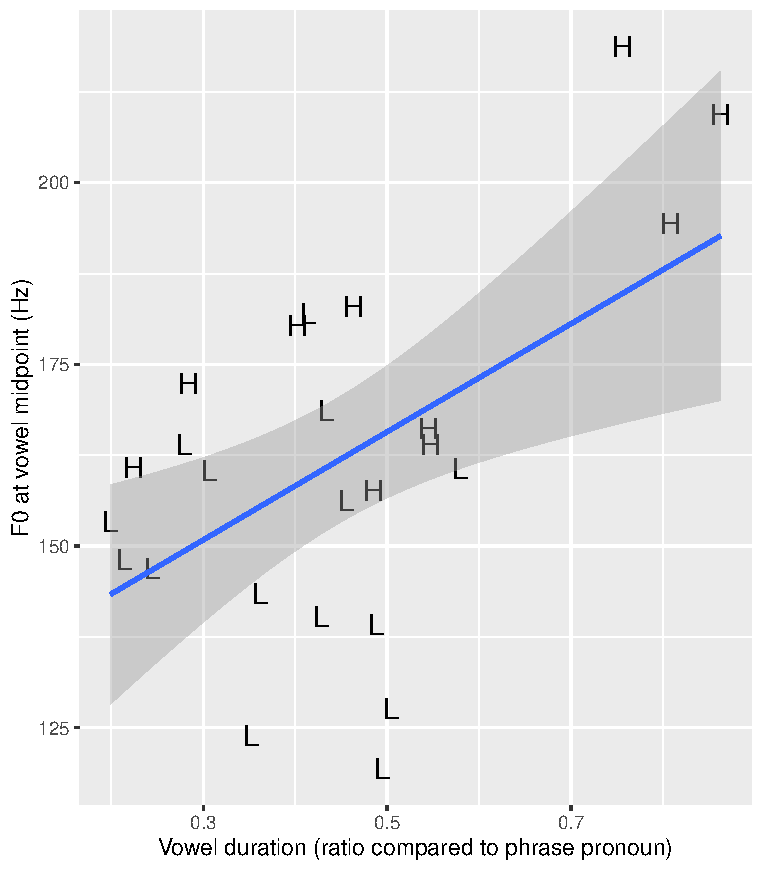
\includegraphics[width=.5\textwidth]{figures/TenutShortVowelsPitchvsDuration.pdf}}%   
     \ffigbox
     {\caption{Nobiin Speaker 1: correlation between mean F0 and vowel duration for phonemically long vowel productions\label{fig:oakley:TenutLongVowelsPitchvsDuration}}}
     {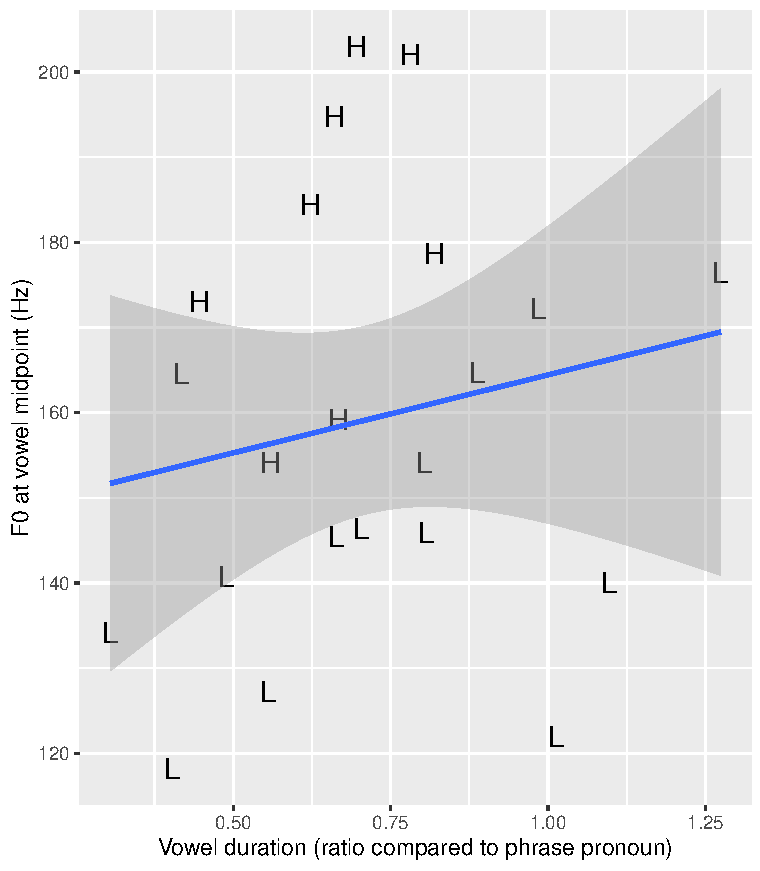
\includegraphics[width=.5\textwidth]{figures/TenutLongVowelsPitchvsDuration.pdf}}
   \end{floatrow}
\end{figure}
   
\begin{figure}
\begin{floatrow}
 \captionsetup{margin=.05\linewidth}
 \ffigbox
 {\caption{Nobiin Speaker 2: correlation between mean F0 and vowel duration for phonemically short vowel productions\label{fig:oakley:NubanShortVowelsPitchvsDuration}}}
 {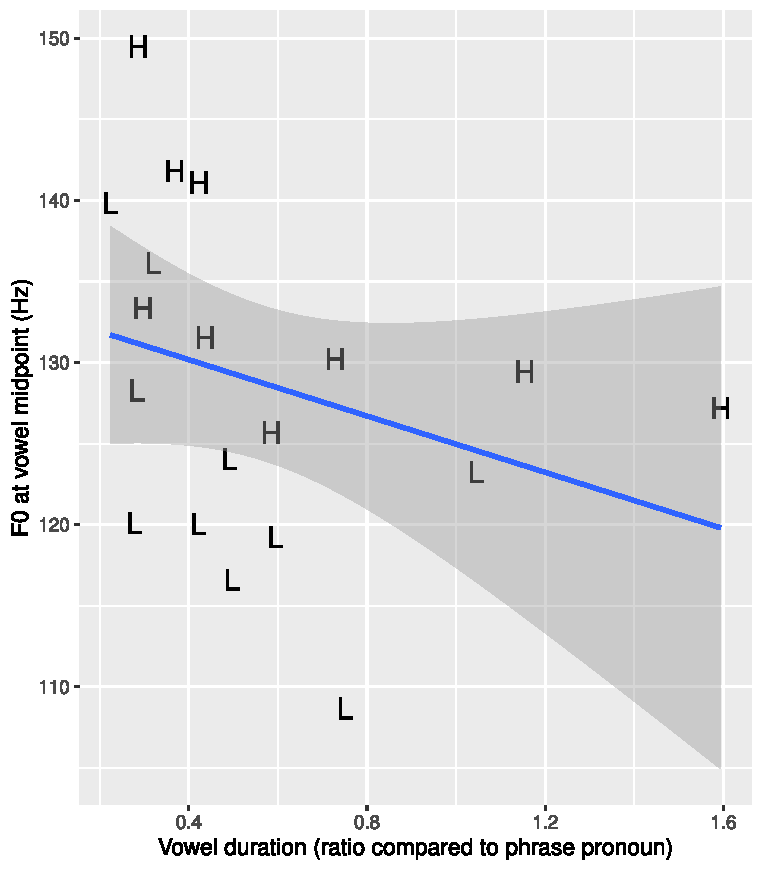
\includegraphics[width=.5\textwidth]{figures/NubanShortVowelsPitchvsDuration.pdf}}%   
 \ffigbox
 {\caption{Nobiin Speaker 2: correlation between mean F0 and vowel duration for phonemically long vowel productions\label{fig:oakley:NubanLongPitchvsDuration}}}
 {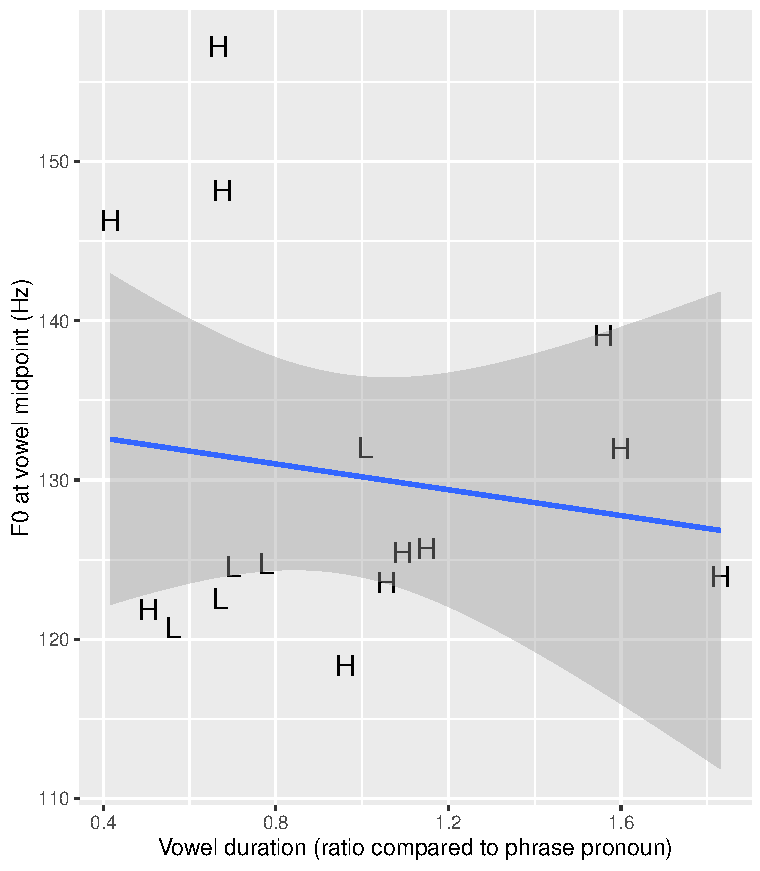
\includegraphics[width=.5\textwidth]{figures/NubanLongPitchvsDuration.pdf}}
\end{floatrow}
\end{figure}

For Nobiin Speaker 1, there is a moderate correlation between mean F0 and vowel duration for phonemically short vowels (Pearson's $r=0.538; p=0.0054$). This shows that pitch and vowel duration are moderately positively correlated for phonemically short vowels. For Speaker 1's phonemically long vowel productions, mean F0 and vowel duration are only weakly correlated (Pearson's $r= 0.179; p=0.423$). Although there is a positive correlation between pitch and vowel duration, the correlation is weak and is not significant.

Nobiin Speaker 2 shows a different pattern from Speaker 1. For Speaker 2's phonemically short vowels, F0 and vowel duration are moderately \textit{negatively} correlated (Pearson's $r= -0.308; p=0.199$), and Speaker 2's phonemically long vowels show a weak negative correlation between F0 and vowel duration (Pearson's $r= -0.148; p=0.583$). Although Speaker 2 shows a negative correlation between pitch and vowel duration, the correlation is not robust for short or long vowels, and is not significant.

\subsection{Guébie acoustic results}
Turning to the Guébie results, we first look at the differences in F0 for the four tone heights. \figref{fig:oakley:olivierTonePitch} and \figref{fig:oakley:borisTonePitch} show the average F0 values in Hz for the four contrastive level tones at three time points.  


\begin{figure}
\begin{floatrow}
 \captionsetup{margin=.05\linewidth}
 \ffigbox
 {\caption{Average F0 measured throughout the vowel for tones 1, 2, 3, and 4 produced by Guébie Speaker 1\label{fig:oakley:olivierTonePitch}}}
 {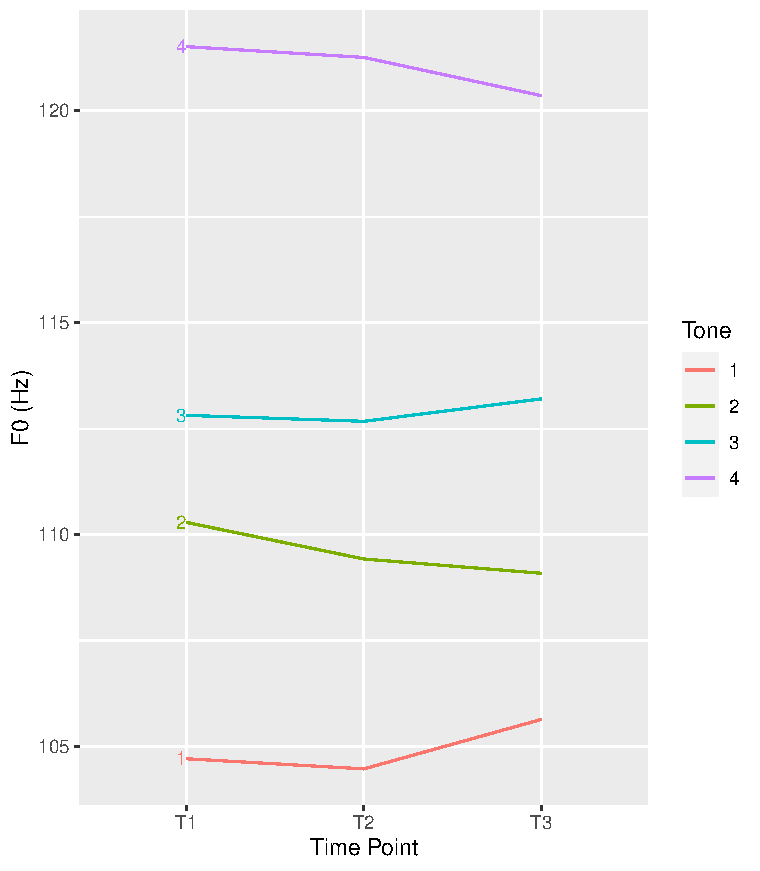
\includegraphics[width=.5\textwidth]{figures/olivierTonePitch.pdf}}%   
 \ffigbox
 {\caption{Average F0 measured throughout the vowel for tones 1, 2, 3, and 4 produced by Guébie Speaker 2\label{fig:oakley:borisTonePitch}}}
 {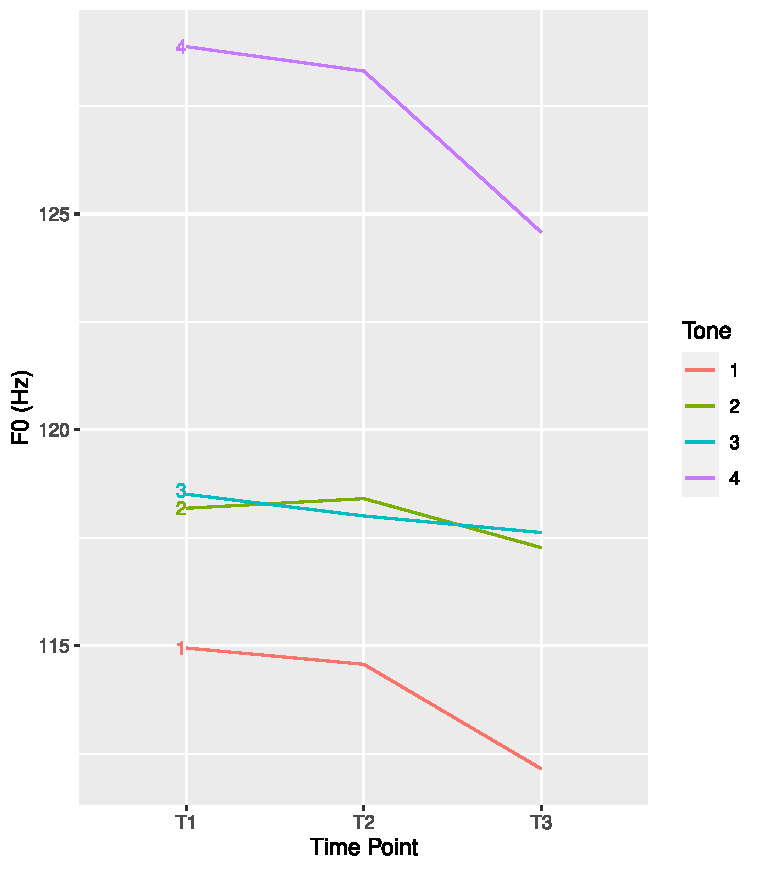
\includegraphics[width=.5\textwidth]{figures/borisTonePitch.pdf}}
\end{floatrow}
\end{figure}

In general, Tone 4 has the highest pitch value at all three time points measured, followed by Tone 3, Tone 2, and finally Tone 1. Exceptionally, Speaker 2's pitch patterns show that Tone 2 rises to the midpoint of the vowel, at which point it has a high pitch value than Tone 3, and then pitch decreases throughout the second half of the vowel.\largerpage

A one-way ANOVA for Speaker 1 and Speaker 2 show a main-effect of tone on pitch at all three measurement points (see \tabref{tab:oakley:GueToneAnova} for results). However, a post-hoc Tukey HSD test confirms that not all tones have significantly different pitch values. First looking at Speaker 1, Tones 1, 2, and 3 do not differ at T1, T2, or T3. Tones 1 and 2 differ from Tone 4 at all three time points. Tone 3 differs from Tone 4 only at T1 and T2, notably caused by a rise in pitch for Tone 3 throughout the duration of the vowel, and a decrease in pitch for Tone 4 throughout the vowel.

\begin{table}
\caption{Results from ANOVAs comparing pitch for Tones 1--4 at 3 time points throughout the vowel}
\label{tab:oakley:GueToneAnova}
\begin{tabular}{l *{2}{S[table-align-text-post=false,table-format=1.2e-1{***}]} S[table-align-text-post=false,table-format=1.5{***}]}
 \lsptoprule
 & {T1} & {T2} & {T3} \\
 \midrule
Speaker 1 & 3.18e-5*** & 1.52e-5*** & 0.0018**  \\ 
Speaker 2 & 3.61e-7*** & 8.96e-6 & 0.00012***  \\ 
\lspbottomrule
\end{tabular}
\end{table}

A post-hoc Tukey HSD test for Speaker 2's ANOVA results show a very similar pattern to Speaker 1. Tone 1, Tone 2, and Tone 3 do not differ in pitch at anytime point, however all three tones differ from Tone 4 at T1, T2, and T3. 

The results are surprising, given both phonetic and phonological evidence that tones are contrastive in Guébie (\cite{sande2020} finds phonetic evidence of pitch differences among tone heights in Guébie, and \cite{sande2017} and \cite{sande2018cross} shows phonological evidence of contrastive level tones in Guébie). There are two explanations that will be explored further here for why the present data may show pitch neutralized across the 4 level tones in Guébie. The first possibility is that the voicing of preceding consonants may impact F0 measurements. \figref{fig:oakley:olivierPitchVoicing} and \figref{fig:oakley:borisPitchVoicing} show the average pitch of Tones 1--4 at the vowel midpoint (T2) following a voiced consonant and a voiceless consonant. A factorial ANOVA for Speaker 1, with F0 as the dependent variable, and preceding voicing and tone as the independent variable, does not show a main effect of preceding consonant voicing on F0 ($p=0.398$), or the interaction between tone and preceding voicing ($p=0.92$). Speaker 2 does appear to have lower pitch on on vowels following voiced consonants than voiceless consonants, particularly for Tones 3 and 4. A factorial ANOVA for speaker 2 does show a main effect of preceding voicing on F0 ($p=0.0058$**). This may explain why Tones 2 and 3 to not differ in F0 for Speaker 2.

\begin{figure}
\begin{floatrow}
 \captionsetup{margin=.05\linewidth}
 \ffigbox
 {\caption{Average F0 at vowel midpoint following voiced and voiceless consonants for Tones1-4 produced by Guébie Speaker 1\label{fig:oakley:olivierPitchVoicing}}}
 {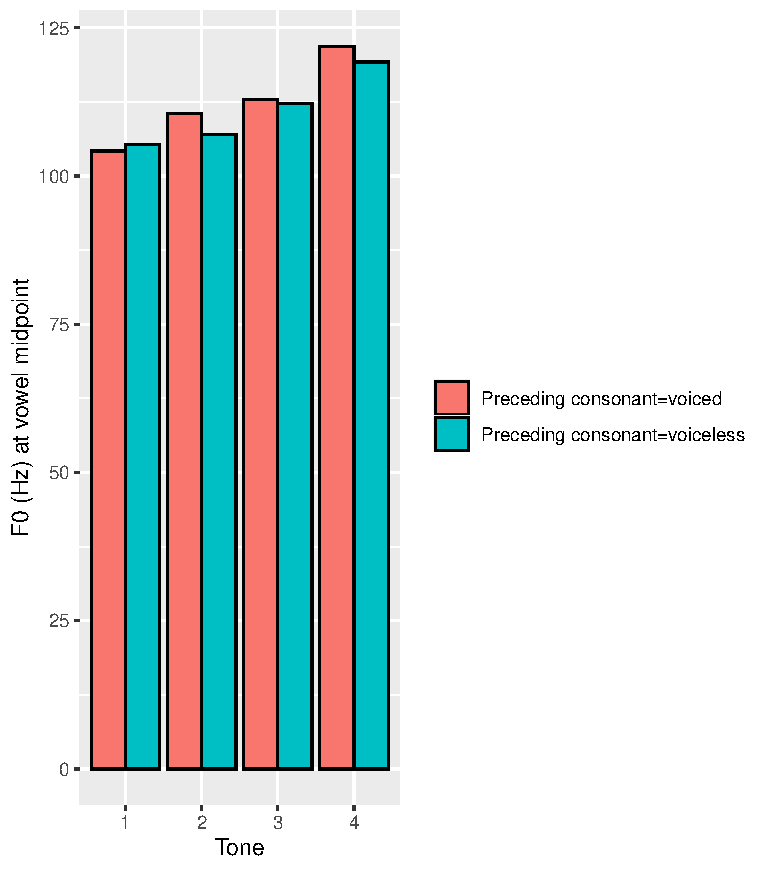
\includegraphics[width=.5\textwidth]{figures/OlivierPitchVoicing.pdf}}%   
 \ffigbox
 {\caption{Average F0 at vowel midpoint following voiced and voiceless consonants for Tones1-4 produced by Guébie Speaker 2\label{fig:oakley:borisPitchVoicing}}}
 {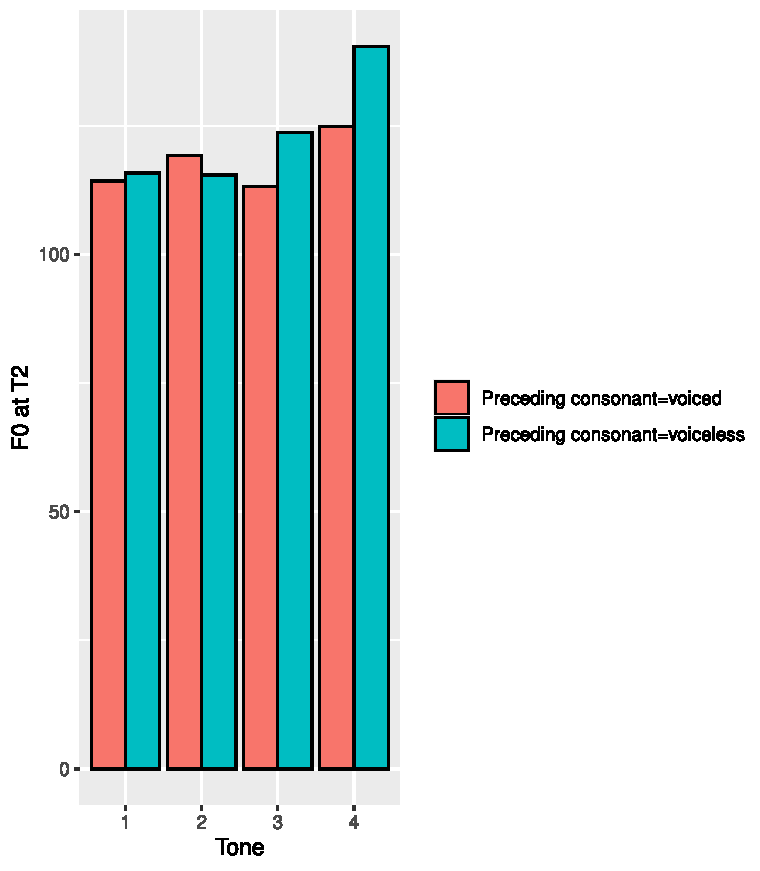
\includegraphics[width=.5\textwidth]{figures/BorisVoicingPitch.pdf}}
\end{floatrow}
\end{figure}

The second possibility is that the phrase position in the carrier phrase of each chosen vowels may interact with intonation. See \sectref{sec:oakley:4} for further discussion on this point.

Next, a logistic mixed-effects model was run in order to reveal which acoustic factors contributed to tone height identity. Tone identity was included as the dependent variable, and F0 at the vowel midpoint, vowel duration, and pitch slope were included as fixed effects. Speaker, vowel quality, and preceding consonant voicing were included as random effects. The output of the model is summarized in \tabref{tab:oakley:GueModel}.

\begin{table}
\caption{Acoustic factors that influence tone height identity; output of logistic-regression model for Guébie speakers\label{tab:oakley:GueModel}}
\begin{tabular}{l S[table-format=1.4{**}]}
 \lsptoprule
Fixed-effect  & {$p$} \\ 
 \midrule
F0 at vowel midpoint & 0.0083**  \\
Pitch slope & 0.286  \\ 
Duration Ratio & 0.403 \\ 
\lspbottomrule
\end{tabular}
\end{table}

The mixed-effects model shows that F0 at the vowel midpoint is a significant factor in predicting tone in Guébie. This result is somewhat expected from results discussed above in \figref{fig:oakley:olivierTonePitch} and \figref{fig:oakley:borisTonePitch}, which shows that tones do differ in F0 (although Tones 1--3 are not significantly different in F0 values. This will be discussed further in \sectref{sec:oakley:4}). The results of the logistic regression, which include vowel quality and preceding consonant voicing as random effects, does find F0 as a significant predictor of tone. Vowel duration and pitch slope, however, are not significant predictors of tone identity.

Finally, the correlation between mean F0 and vowel duration was measured in order to describe the relationship between these two acoustic measurements. The correlation of vowel duration and pitch are shown in \figref{fig:oakley:olivierPitchDurationCorrelation} for Guébie Speaker 1, and the correlation of vowel duration and pitch are shown in \figref{fig:oakley:borisPitchDurationCorr} for Guébie Speaker 2.

\begin{figure}
\begin{floatrow}
 \captionsetup{margin=.05\linewidth}
 \ffigbox
 {\caption{Guébie Speaker 1: correlation between mean F0 and vowel duration vowel productions\label{fig:oakley:olivierPitchDurationCorrelation}}}
 {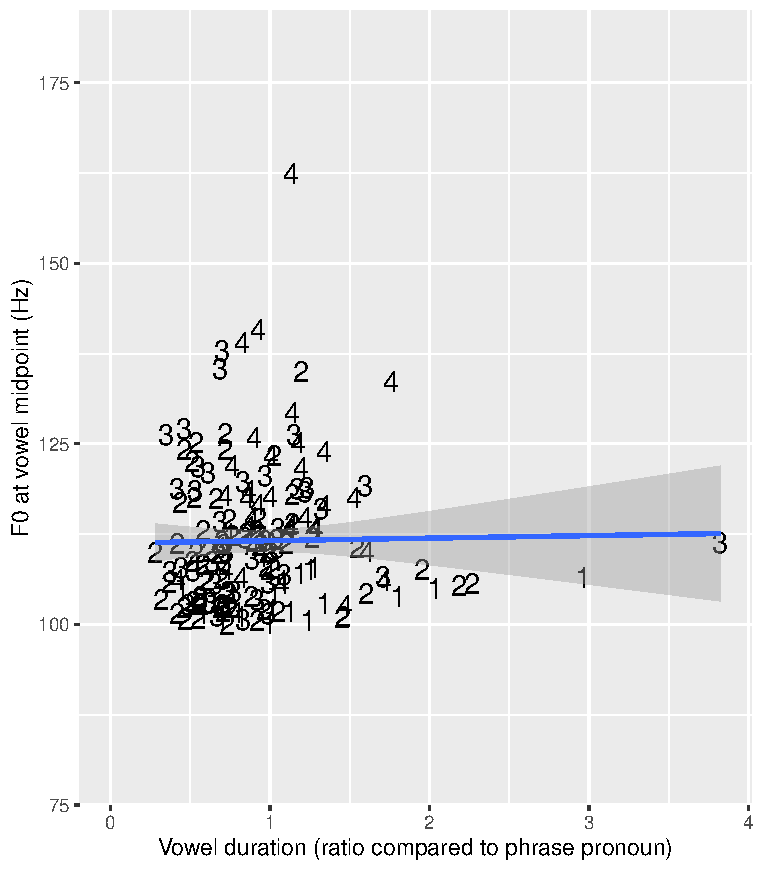
\includegraphics[width=.5\textwidth]{figures/olivierPitchDurationCorrelationScatter.pdf}}%   
 \ffigbox
 {\caption{Guébie Speaker 2: correlation between mean F0 and vowel duration vowel productions\label{fig:oakley:borisPitchDurationCorr}}}
 {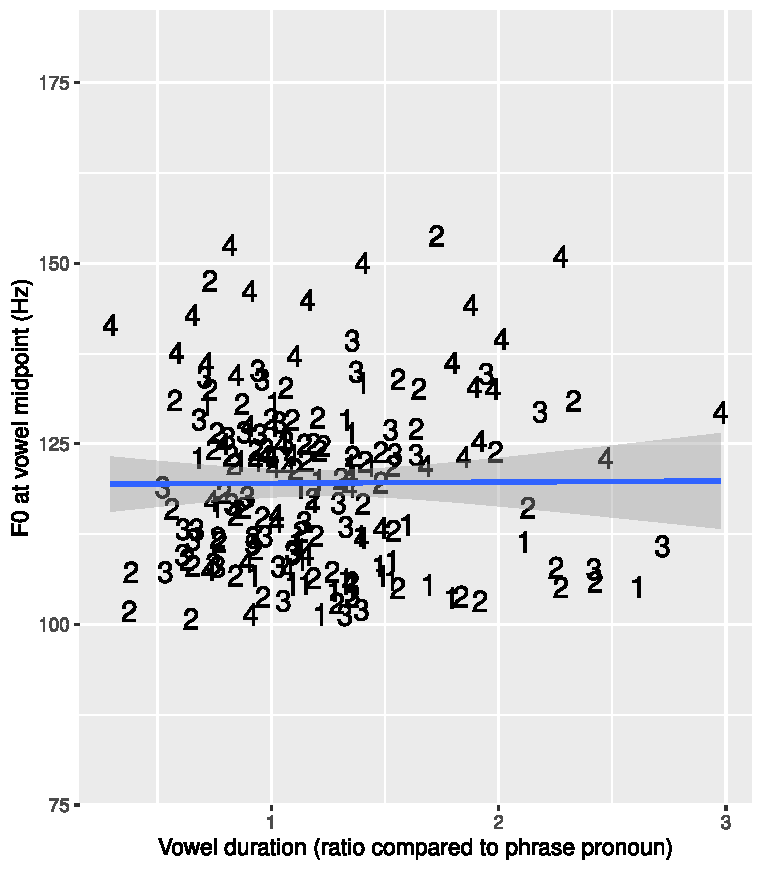
\includegraphics[width=.5\textwidth]{figures/borisPitchDurationCorrScatter.pdf}}
\end{floatrow}
\end{figure}
   
The results for Guébie Speaker 1 show a very weak positive correlation between vowel duration and F0 at the vowel midpoint (Pearson's $r=0.019; p=0.8$). This weak correlation does not appear to be driven by the outliers in the data, specifically by the vowels with a particularly long vowel duration. Removing the 5 tokens that are 2 standard deviations above the mean vowel duration (which is 0.96 of the duration of the pronoun vowel) yields only a slightly stronger positive correlation between F0 and vowel duration ($r=0.243; p=0.24$). Speaker 2 shows similar results. F0 and the vowel midpoint and vowel duration ratio are weakly positively correlated (Pearson's $r=0.022; p=0.76$). Taken together, although there is a slight trend for pitch and vowel duration to be positively correlated in Guébie, there is not strong evidence for a correlation.

\section{Discussion}\label{sec:oakley:4}
This study found pitch to be the primary acoustic correlate to tone in Nobiin, a language with two contrastive tone heights and phonemic vowel length, and Guébie, a language with 4 contrastive level tones. There is little evidence that vowel duration varies according to pitch in either language, despite suggestions that pitch and duration tend to be negatively correlated. \sectref{sec:oakley:1} of this study outlined three research questions, which we return to here.

The first research question of this study was to examine the relationship between vowel length and tone. First, the results from \sectref{sec:oakley:3} show that H tones tended to have a \textit{longer} duration than L tones. Second, there is no evidence that long vowels differed from short vowels in F0 at the vowel midpoint for either speaker, showing that F0 does not appear to be used to enhance the contrast between short and long vowels.

The second research question asked what the acoustic correlates to tone were for Nobiin and Guébie. A logistic regression with tone as the dependent variable finds that F0 at the vocalic midpoint is a predictor of tone identity in Nobiin and in Guébie, but vowel duration and pitch slope are not. It could by hypothesized that tonal contrasts in Guébie would be more likely to make use of both duration and pitch cues to enhance the contrasts (because vowel length is not used contrastively in Guébie), whereas vowel duration is not an optimal correlate to tone in Nobiin (because vowel length is contrastive). However, only pitch correlates to tonal contrasts in both languages, despite the different status of phonological vowel length in the two languages.


A further note must be made here regarding the acoustics of tone in Guébie. As mentioned in \sectref{sec:oakley:3}, the results of a one-way ANOVA here did not show a significant difference in F0 value of tones 1-3 throughout most of the vowel. This result is surprising given previous findings \citep{sande2018cross, sande2020}. Again, this result is likely not entirely attributable to the effects of the preceding consonant voicing, given that only Speaker 2 shows an effect of preceding consonant voicing on F0 value. The second alternative is that this phonetic finding is an effect of intonation. The present study only examines tones in phrase medial position, usually at the verb phrase boundary, which allows duration normalization with the pronoun, and increased similarity to the carrier phrase structure elicited with the Nobiin speakers. There is suspected to be a boundary tone in Guébie (Sande, p.c.) that may cause tone lowering at phrasal boundaries. Because this study excluded all phrase initial vowels, the pitch differences between the vowels may have been neutralized. Although describing the intonational system of Guébie is outside the scope of the present study, these results show interesting findings compared to previous work on Guébie acoustics, and more work on the acoustics of suprasegmentals in underdocumented languages should be undertaken.

The final research question posed whether there was a negative or positive correlation between pitch and vowel duration in Nobiin and Guébie. This study does not find evidence for a universal negative correlation between pitch and duration, as has been suggested in previous studies \citep{gandour1977interaction, dreher1968instrumental}. For Nobiin, Speaker 1 shows a positive correlation between vowel duration and pitch, while Speaker 2 shows a very weak negative correlation between vowel duration and pitch. Despite the fact that the two speakers show different patterns, these results do not support the hypothesis that there is a universal negative correlation between pitch and duration. Similarly, the Guébie speakers do not show evidence for a negative correlation between pitch and vowel duration. These results support the notion that the correlation between these phonetic features may be language, or even speaker, specific. 

Taken together, this study finds that Nobiin and Guébie evidence that F0, but not vowel length or pitch slope, is an acoustic correlate to level tones. For Nobiin, vowel duration is an acoustic correlate to vowel length, but not tone. It has been discussed that when vowel duration is a contrastive phonological feature of a language, duration may not be an active phonetic cue to prominence \citep{remijsen2014study}. The findings of the present study show that tonal languages with and without contrastive vowel length do \textit{not} use vowel duration as a secondary acoustic correlate to tone. Even in languages without contrastive vowel length, vowel duration is not necessarily used to enhance tonal contrasts. Although this finding is preliminary, it motivates future work exploring the acoustic correlates to tone and vowel length in languages that use both contrastively.


\section{Limitations}
One limitation to the present study is the small sample of speakers representing Nobiin and Guébie. Gathering phonetic data from a large number of speakers is not feasible. For Nobiin, speakers have been displaced, making it difficult to work with a large group of native speakers. For Guébie, very few speakers live outside of C\^ote d'Ivoire, making it necessary to travel to collect recordings. In the villages where Guébie is spoken, there is social pressure to work with male speakers, rather than female speakers, and only certain male speakers are willing to participate in individual recording sessions. Despite the limitations on the small sample size of the speakers from each language, this research represents the first time acoustic correlates to tone in Nobiin or Guébie has been documented, adding to a diversity of language data represented in the phonetic literature.


\section{Conclusion}
This study investigates the acoustic properties of lexical tone in two understudied African languages, Nobiin and Guébie. Nobiin has two contrastive level tones realized as H and L on the surface, and phonological vowel length. Guébie has four contrastive level tones and no phonological vowel length. The results of production tasks show that pitch is the primary acoustic correlate to tone in both Nobiin and Guébie. These results have implications for the phonetics-phonology interface, and show that vowel length is not used as an acoustic correlate to tone in these two languages, regardless of the phonological status of vowel length. As for the correlation between these acoustic features, there is evidence for a positive correlation between pitch and duration in both languages. These results support more recent findings that argue that the assumed universal negative correlation between pitch and duration is, in fact, language specific (perhaps even speaker specific) which further highlights the importance of including a wider range of understudied languages in phonetic research.


\section*{Abbreviations}
\begin{multicols}{2}\raggedcolumns
\begin{tabbing}
Hz\hspace{1ex} \= Hertz\kill
$\emptyset$ \> Null tone \\
1 \> First person \\
F0 \> Fundamental frequency  \\
H \> High tone  \\ 
Hz \> Hertz \\
L \> Low tone \\ 
M \> Mid tone \\
ms \> Milliseconds\\
sg \> Singular \\
T1 \> First time point \\
T2 \> Second time point \\
T3 \> Third time point\\
\end{tabbing}
\end{multicols}

\section*{Acknowledgments}
I would like to thank Georgetown University's PhonLab for their feedback on this work. Thank you to Hannah Sande, Maya Barzilai, Alexandra Pfiffner, Elizabeth Zsiga, and Katherine Russel for their insights. I would also like to thank the Guébie and Nobiin communities for all their time spent working on this project.


{\sloppy\printbibliography[heading=subbibliography,notkeyword=this]}
\end{document}
